\chapter{Macchine eoliche}
\section{Il teorema di Betz}
Il primo a studiare scientificamente le turbine eoliche fu l'ingegnere e fisico tedesco Albert Betz, il quale, attraverso una serie di ragionamenti giunse a determinare la massima potenza estraibile da un flusso d'aria.

Il teorema di Betz è tanto fondamentale per le macchine eoliche quanto quello di Carnot per le macchine termiche. 

La teoria di Betz si fonda su due postulati
\begin{itemize}
\item il flusso attraversante un'immaginaria sezione $S_1$ di una turbina, a monte del piano di rotazione della stessa, possiede velocità $V_1$;
\item il flusso in una sezione $S_2$, a valle della turbina, possiede una velocità $V_2$.
\end{itemize}
\begin{figure}
\centering
  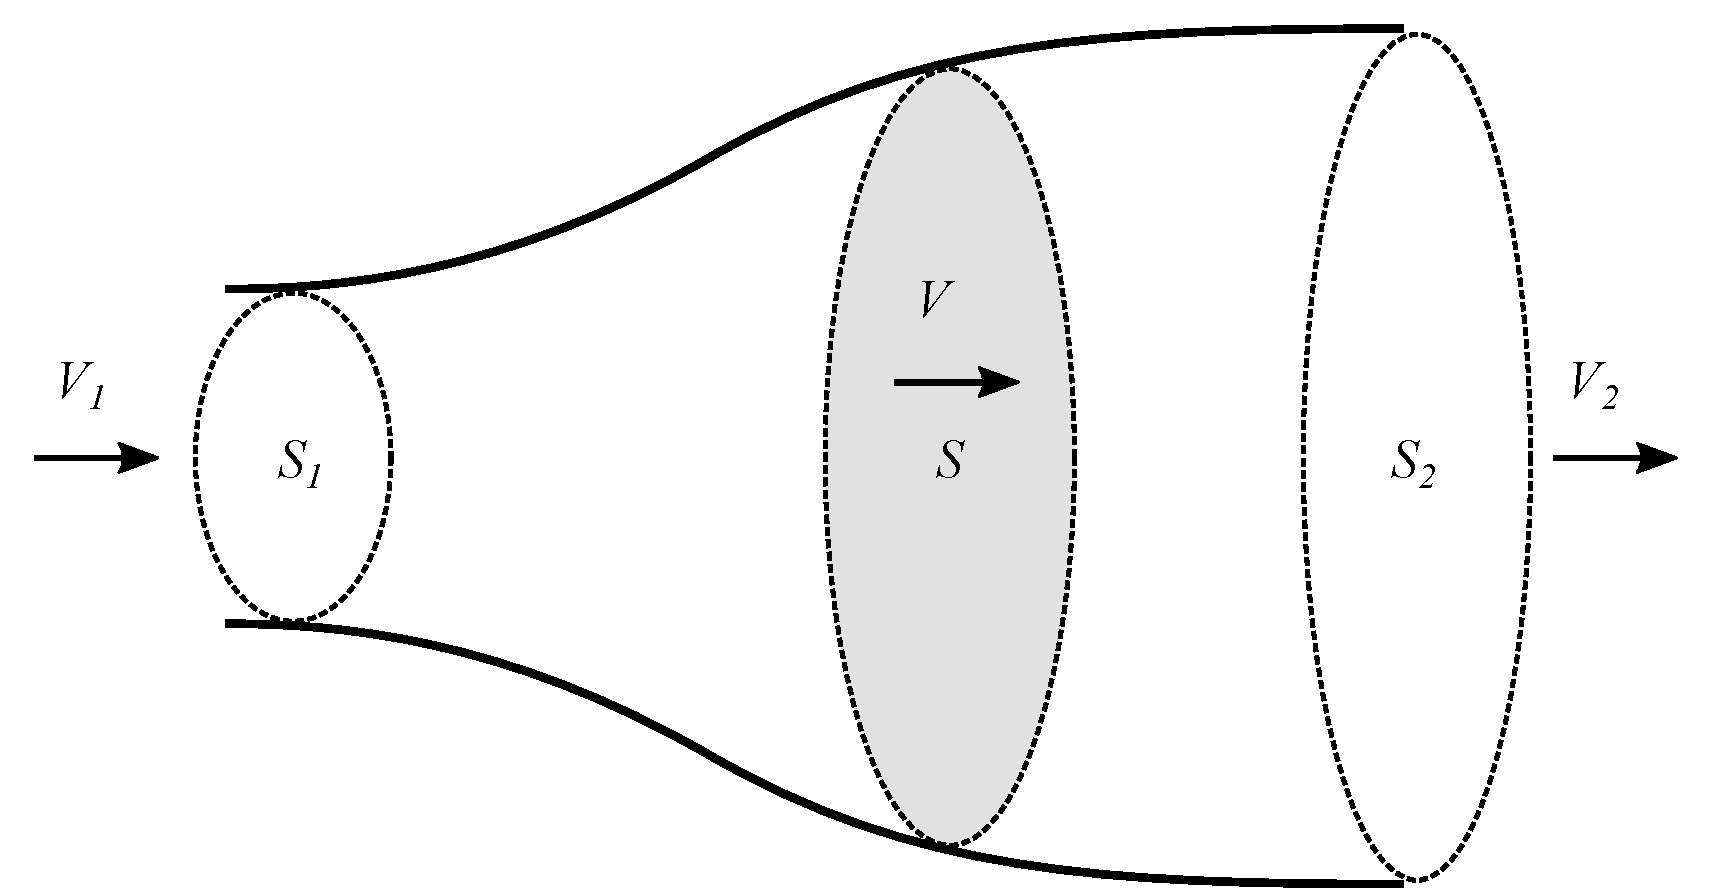
\includegraphics[width=.6\textwidth]{fig/Betz.pdf}
\caption{}
\label{}
\end{figure}
Nella realtà, il flusso a valle della turbina è vorticoso, fatto che complica molto l'analisi, per cui l'ipotesi semplificativa di Betz consiste nell'assumere che la rotazione della turbina non trasmetta al fluido alcun moto in senso tangenziale. In ultima analisi, il flusso è bidimensionale e le sue componenti assiali e radiali. 

In virtù del Principio di Conservazione dell'Energia, se una turbina estrae una certa quantità di energia da un flusso d'aria, questo deve cedere la stessa quantità di energia cinetica. Pertanto, la velocità $V_2$ deve essere inferiore alla velocità $V_1$. Se supponiamo che l'aria è incomprimibile, allora si deve soddisfare l'equazione di continuità
\begin{align*}
S_1 \cdot V_1 = S_2 \cdot V_2 = S \cdot V
\end{align*}
La sezione $S$ indica la superficie spazzata dalla rotazione dell'elica.
Se valutiamo la forza $F$ esercitata dalla turbina sul flusso d'aria in movimento, per l'equazione di Eulero, il suo valore assoluto è dato dalla seguente espressione:
\begin{align*}
F = Q \cdot \left( V_1 - V_2 \right) = S \cdot V \cdot \rho \cdot \left( V_1 - V_2 \right)
\end{align*}
dove:\\
$F$ = Valore assoluto della forza $[N]$\\
$\rho$ = densità dell'aria ($1.2$ a $1.25$ $kg/m^3$)\\
$Q$ = portata del flusso d'aria $[kg/s]$\\
$V_1$ = velocità dell'aria a monte della turbina $[m/s]$\\
$V_2$ = velocità dell'aria a valle della turbina $[m/s]$\\
$V$ = velocità dell'aria che passa attraverso la turbina $[m/s]$\\[2mm]
La potenza P assorbita dalla turbina è data da 
\begin{equation}\label{eq:potEol}
P = F \cdot V = \rho \cdot S \cdot V^2 \cdot \left( V_1 - V_2 \right)
\end{equation}
Se ora consideriamo la potenza assorbita dalla turbina come la variazione di energia cinetica della massa d'aria $\Delta E$, passante attraverso la sezione $S$ della turbina per ogni secondo, avremo la seguente espressione:
\begin{equation}\label{enEol}
\Delta E = \frac{1}{2} \rho	S V \left(V_1 - V_2 \right) = P
\end{equation}
Eguagliando \ref{enEol} con \ref{eq:potEol} si ottiene:
\begin{align*}
P = \rho S V^2 \left(V_1 - V_2 \right) = \frac{1}{2} \rho S V \left(V_1^2-V_2^2 \right)
\end{align*}
\begin{align*}
V \left(V_1 - V_2 \right) = \frac{1}{2} \left(V_1^2-V_2^2 \right) = \frac{1}{2} \left(V_1-V_2 \right)\left(V_1+V_2 \right)
\end{align*}
Semplificando 
\begin{equation}\label{eq:vmedia}
V = \frac{V_1 + V_2}{2}
\end{equation}
Sostituendo la \ref{eq:vmedia} nella \ref{eq:potEol} si ottiene la seguente espressione:
\begin{equation}\label{eq:potfin}
P = \frac{1}{4} \rho S \left( V_1 +V_2 \right) \cdot \left(V_1^2 - V_2^2 \right)
\end{equation}
Assumendo $V_1$ costante si può poi calcolare il valore di $V_2$ che massimizza la potenza, derivando l'equazione \ref{eq:potfin} e ponendola a $0$. 
\begin{align*}
\frac{dP}{dV_2} = \frac{1}{4} \rho S \left( V_1^2 - 2 V_1 V_2 - 3 V_2^2 \right) = 0
\end{align*}
Si tratta di un'equazione quadratica che ammette due radici, una è negativa e non ha significato fisico. Si ottiene
\begin{align*}
V_{2,ott} = \frac{V_1}{3}
\end{align*}
Sostituendo l'espressione appena ricavata nell'espressione di $P$ si ottiene la potenza massima estraibile
\begin{align*}
P_{max} = \frac{8}{27} \rho S V_1^3 
\end{align*}

\section{Definizione del problema}
L'aria passando attraverso una turbina eolica in movimento, perde velocità nel veso del flusso. Siccome le turbine degli aerogeneratori sono sprovviste di alette direzionali o deflettori, il movimento di rotazione delle pale genera una componente tangenziale nel moto dell'aria. L'espansione del flusso genera invece una componente radiale che è stato dimostrato essere trascurabile. 

Per la progettazione di una mini o microturbina eolica ci si può avvalre di una teoria semplificata la cui validità è stata dimostrata per via empirica. Si effettuano le seguenti ipotesi di lavoro:
\begin{enumerate}
\item le condizioni indisturbate a monte della turbina sono velocità $V_1$ e pressione $p_0$;
\item le condizioni asintotiche a valle della turbina sono velocità $V_2 < V_1$, moto rotazionale con velocità angolare $\omega$
\item un infinitesimo a monte del piano di rotazione della turbina, la pressione è $P$, la velocità sull'asse delle $x$ è $V$ e la rotazione delle pale con velocità angolare $\Omega$ induce sull'aria un moto rotazionale con la stessa velocità angolare;
\item un infinitesimo a valle del piano di rotazione della turbina, la pressione $P_1$, la velocità sull'asse delle $x$ è sempre $V$, ma il moto rotazionale indotto sull'aria ha una velocità angolare pari a $\Omega+\omega$;
\item si analizzano i flussi d'aria attraverso un'area differenziale $dS$, situata ad una distanza generica $r$ dall'asse di rotazione della turbina. Lo spessore di questo anello differenziale è $dr$.
\end{enumerate}
\begin{figure}
\centering
  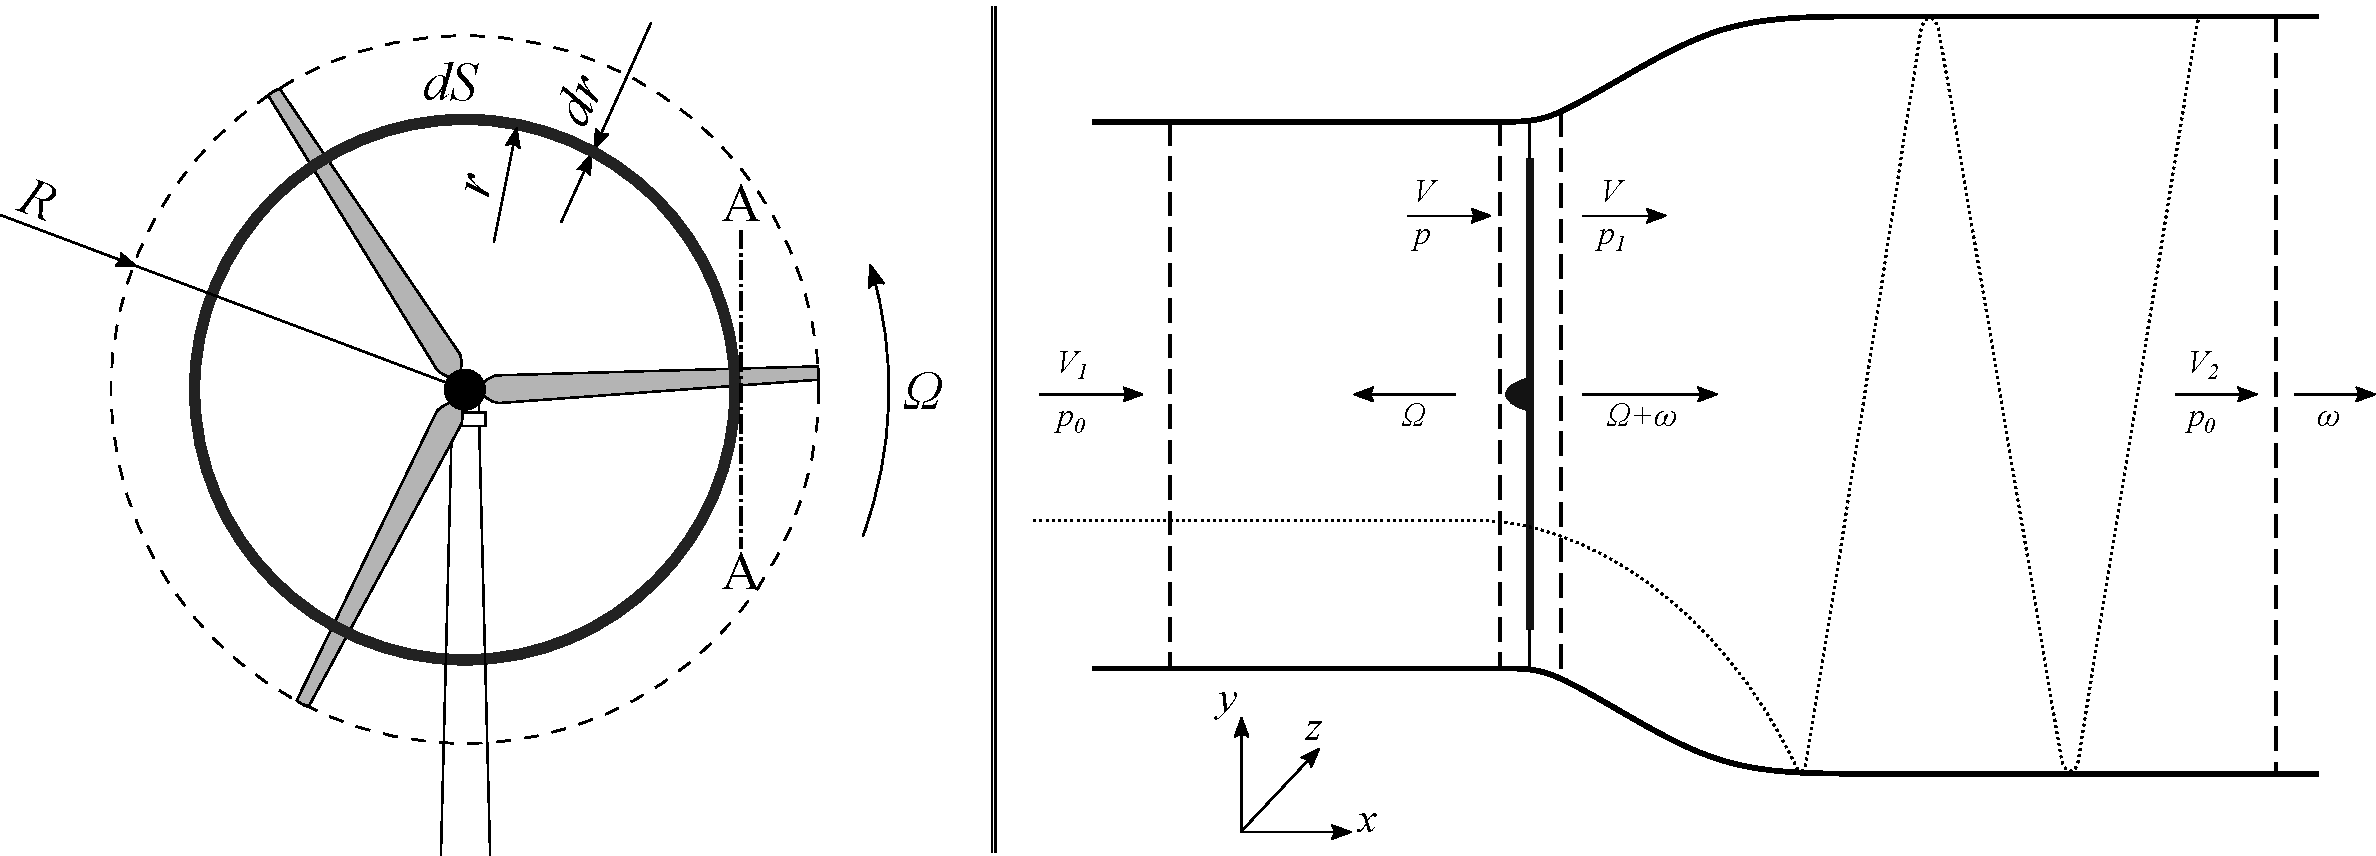
\includegraphics[width=\textwidth]{fig/frontlatEol.pdf}
\caption{A sinista la turbina vista dal lato monte, a destra la vista laterale.}
\label{fig:frontlatEol}
\end{figure}
\begin{figure}
\centering
  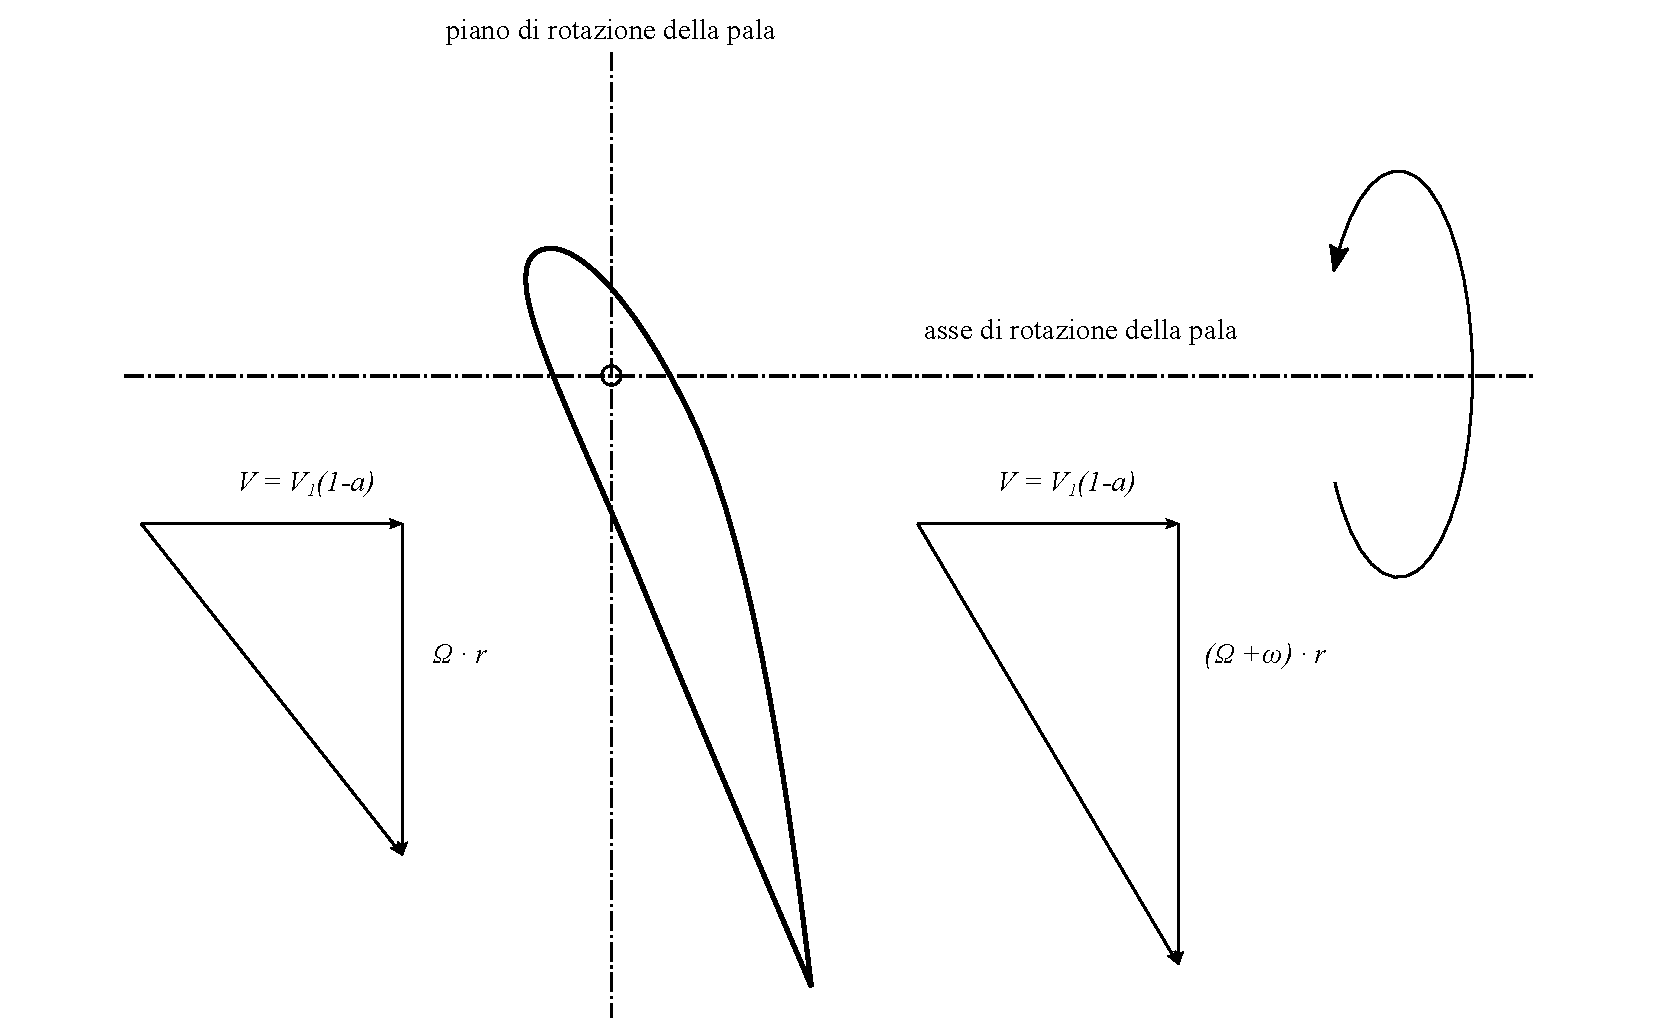
\includegraphics[width=\textwidth]{fig/triangEol.pdf}
\caption{Composizione delle velocità in un elemento di pala generico dell'elica in movimento (corrispondente alla sezione A-A della figura \ref{fig:frontlatEol})}
\label{fig:triangEol}
\end{figure}
Per calcolare la potenza sviluppata da un elemento differenziale di pala, si utilizzano le equazioni di conservazione della quantità di moto, si potrà così integrare per la lunghezza della pala per ricavare la potenza totale. Conoscendo la potenza massima ottenibile, si potranno definire, in ogni punto della pala, corda e angolo di attacco del profilo. 

Bisogna prima definire dei coefficienti ausiliari che verranno utlizzati nei calcoli. 

La velocità attraverso l'elica $V_1$ non è nota a priori, risulta utile definire un coeficiente adimensionale che consenta di esprimere $V$ in funzione della velocità del vento a monte della pala. Si definisce 
\begin{equation}\label{eq:coeff_a}
a = 1-\frac{V}{V_1} \;\; \Rightarrow \;\; V = V_1 \cdot \left(1-a \right)
\end{equation}
Uguagliamo ora la \ref{eq:coeff_a} con la \ref{eq:vmedia}
\begin{align*}
V = V_1 (1-a) = \frac{V_1 +V_2}{2}
\end{align*}
\begin{align*}
2 V_1 (1-a) - V_1 = V_2
\end{align*}
\begin{align*}
V_2 = V_1 (1-2a)
\end{align*}
\subsection{Coefficiente di perdita di velocità}
Il coefficiente $a$ permette di calcolare alcune velocità in funzione di altre secondo convenienza. Il valore di $a$ non è noto a priori, si sa che deve essere compreso tra $0 \leq a \leq 1/2$ e idealmente si deve avere $a = 1/3$\footnote{Dal teorema di Betz}. Un valore pari a $1/2$ renderebbe nulla la $V_2$, condizione fisicamente impossibile. Una condizione $a=0$ implicherebbe $V_2 = V_1$ (turbina frenata). 
\subsection{Coefficiente di velocità specifica locale}
Si definisce ora il coefficiente di velocità specifica locale all'estremità della pala 
\begin{align*}
\lambda = \frac{u}{V_1} = \frac{\Omega R}{V_1} 
\end{align*}
Lo stesso coefficiente per un punto $r$ generico lo posso esprimere in funzione di $\lambda$
\begin{align*}
\lambda_r = \frac{\Omega \cdot r}{V_1} = \frac{\lambda \cdot r}{R} 
\end{align*}
\subsection{Coefficiente di velocità angolare}
La velocità angolare della turbina è pari a $\Omega$. L'interazione delle pale del rotore con l'aria introduce su quest'ultima una componente rotazionale, la cui velocità angolare è pari a $\omega$. Si definisce la relazione tra dette velocità angolari come 
\begin{align*}
a' = \frac{\omega}{2 \Omega}
\end{align*}

\section{Teoria del tubo di flusso anulare con scia vorticosa}
Si vogliono trovare le relazioni che legano $a$, $a'$ e $\lambda$. Conoscendo tali relazioni si possono rivavare i valori di $V_1$, $V_2$ e $\omega$. 
Facendo riferimento alla figura \ref{fig:frontlatEol} si applica il teorema di Bernoulli tra una sezione posta infinitamente a monte della turbina e una posta un infinitesimo a monte. Si ottiene
\begin{align*}
p_0 + \frac{\rho V_1}{2} = p + \frac{\rho V}{2}
\end{align*}
Applichiamo ora il teorema tra una sezione infinitesimalmente a valle della turbina e una infinitamente a valle\\
\begin{align*}
p_0 + \frac{\rho V_2}{2} = p_1 + \frac{\rho V}{2}
\end{align*}
Sottraendo membro a membro si ottiene
\begin{align*}
\frac{\rho V_1^2}{2} . \frac{\rho V_2^2}{2} = p - p_1 = \Delta p
\end{align*}

\begin{figure}
\centering
  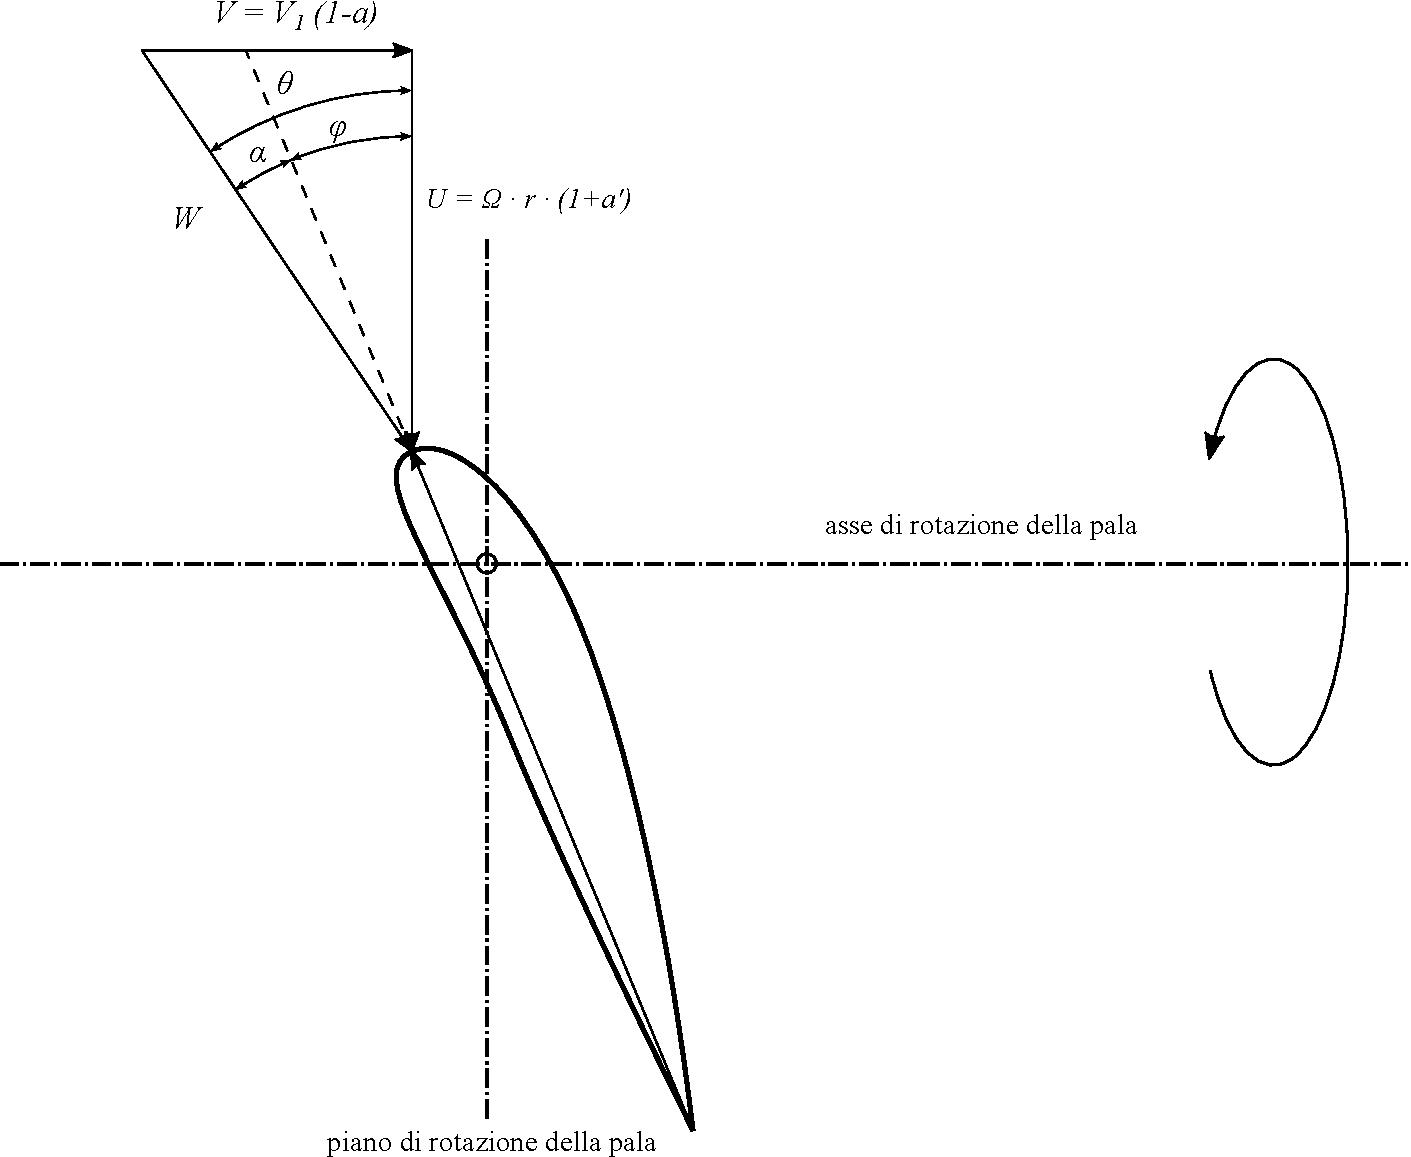
\includegraphics[width=\textwidth]{fig/triangEol2.pdf}
\caption{}
\label{fig:triangEol2}
\end{figure}